%% This is file `elsarticle-template-3-num.tex',
%%
%% Copyright 2009 Elsevier Ltd
%%
%% This file is part of the 'Elsarticle Bundle'.
%% ---------------------------------------------
%%
%% It may be distributed under the conditions of the LaTeX Project Public
%% License, either version 1.2 of this license or (at your option) any
%% later version.  The latest version of this license is in
%%    http://www.latex-project.org/lppl.txt
%% and version 1.2 or later is part of all distributions of LaTeX
%% version 1999/12/01 or later.
%%
%% given in the file `manifest.txt'.
%%
%% Template article for Elsevier's document class `elsarticle'
%% with numbered style bibliographic references
%%
%% $Id: elsarticle-template-3-num.tex 165 2009-10-08 07:58:10Z rishi $
%% $URL: http://lenova.river-valley.com/svn/elsbst/trunk/elsarticle-template-3-num.tex $
%%
%\documentclass[preprint,12pt]{elsarticle}

%% Use the option review to obtain double line spacing
%% \documentclass[preprint,review,12pt]{elsarticle}

%% Use the options 1p,twocolumn; 3p; 3p,twocolumn; 5p; or 5p,twocolumn
%% for a journal layout:
%% \documentclass[final,1p,times]{elsarticle}
%% \documentclass[final,1p,times,twocolumn]{elsarticle}
%% \documentclass[final,3p,times]{elsarticle}
%% \documentclass[final,3p,times,twocolumn]{elsarticle}
\documentclass[final,5p,times]{elsarticle}
%% \documentclass[final,5p,times,twocolumn]{elsarticle}

%% if you use PostScript figures in your article
%% use the graphics package for simple commands
%% \usepackage{graphics}
%% or use the graphicx package for more complicated commands
 \usepackage{graphicx}
%% or use the epsfig package if you prefer to use the old commands
%% \usepackage{epsfig}

%% The amssymb package provides various useful mathematical symbols
\usepackage{amssymb}
\usepackage{amsmath}
%% The amsthm package provides extended theorem environments
%% \usepackage{amsthm}

%% The numcompress package shorten the last page in references.
%% `nodots' option removes dots from firstnames in references.
\usepackage[nodots]{numcompress}

%% The lineno packages adds line numbers. Start line numbering with
%% \begin{linenumbers}, end it with \end{linenumbers}. Or switch it on
%% for the whole article with \linenumbers after \end{frontmatter}.
\usepackage{lineno}

%% Avoids linenumbers to collide with text for 5p format:
\setlength\linenumbersep{3pt}

%% natbib.sty is loaded by default. However, natbib options can be
%% provided with \biboptions{...} command. Following options are
%% valid:

%%   round  -  round parentheses are used (default)
%%   square -  square brackets are used   [option]
%%   curly  -  curly braces are used      {option}
%%   angle  -  angle brackets are used    <option>
%%   semicolon  -  multiple citations separated by semi-colon
%%   colon  - same as semicolon, an earlier confusion
%%   comma  -  separated by comma
%%   numbers-  selects numerical citations
%%   super  -  numerical citations as superscripts
%%   sort   -  sorts multiple citations according to order in ref. list
%%   sort&compress   -  like sort, but also compresses numerical citations
%%   compress - compresses without sorting
%%
%% \biboptions{comma,round}

% \biboptions{}


\journal{Computers \& Graphics}

\begin{document}

\begin{frontmatter}

%% Title, authors and addresses

%% use the tnoteref command within \title for footnotes;
%% use the tnotetext command for the associated footnote;
%% use the fnref command within \author or \address for footnotes;
%% use the fntext command for the associated footnote;
%% use the corref command within \author for corresponding author footnotes;
%% use the cortext command for the associated footnote;
%% use the ead command for the email address,
%% and the form \ead[url] for the home page:
%%
%% \ title{Title\tnoteref{label1}}
%% \tnotetext[label1]{}
%% \ead{email address}
%% \ead[url]{home page}
%% \fntext[label2]{}
%% \cortext[cor1]{}
%% \address{Address\fnref{label3}}
%% \fntext[label3]{}

\title{Procedural Bread Making}

%% use optional labels to link authors explicitly to addresses:
%% \author[label1,label2]{<author name>}
%% \address[label1]{<address>}
%% \address[label2]{<address>}

\author{}

\address{}

\begin{abstract}
%% Text of abstract
Photorealistic rendering real scenes has been a core target of computer graphics since its begginings. However, little efforts have been devoted to the accurate rendering of food. In this paper we present an accurate computational bread making model which allows to faithfully represent the geometrical structure and the appearance of baked bread. We achieve this by a careful simulation of the conditions during proving, baking and kneading to get a realistically looking bread. Our results are successfully compared to real bread by both visual inspection and by a multi-fractal-based error metric.
\end{abstract}

\begin{keyword}
Bread \sep Photorealism \sep Fractal \sep Procedural
%% keywords here, in the form: keyword \sep keyword

%% MSC codes here, in the form: \MSC code \sep code
%% or \MSC[2008] code \sep code (2000 is the default)

\end{keyword}

\end{frontmatter}

%%
%% Start line numbering here if you want
%%
\linenumbers

%% main text
%====================================================================
%====================================================================
%====================================================================
\section{Introduction}
% ================ What is knwon
Since its very begginings, Computer Graphics has aimed at achieving photorealistic modeling and rendering of real-world scenes~\cite{Hughes2013}. There have been tremendous efforts to produce realistic results for a large variety of scenes, from natural to synthetic scenes, and from natural landscapes to urban scenarios. This has resulted in spectacular models to represent almost everything, from water to fire, and from clouds to concrete.

% ================ what is unknown
However, not much attention has been paid to modeling and rendering of food beyond some sparse efforts~\cite{Tong2005,Cho2007}. In particular, accurately modeling bread and its baking process has attracted a lot of attention for food engineering (e.g., \cite{Purlis2010}), but there are no equivalent efforts for translating this research into the graphics community.

% ================ Our burning question
In this paper we aim to faithfully simulate the different stages that bread undergo during its cooking process: proving, baking and kneading. For that, we use state-of-the-art techniques from food engineering to solve the equations of the first two processes, we add gas bubbles to the model to generate crumbs, and finally we add a user provided kneading stage that allows the user to freely warp the resulting bread. The resulting bubble and crust distribution faithfully reproduce the appearance of real bread.

%====================================================================
%====================================================================
%====================================================================
\section{Previous Work}
Accurate geometric models are main requirements in material modeling and rendering \cite{Dorsey2007}. 

Procedural modeling of geometry avoids the need for artistical intervention in impractical domains: cities \cite{Parish2001}, planets \cite{Ebert2002}, buildings \cite{Muller2006}, and plants \cite{Prusinkiewicz1990}. These methods use grammars to define mathematical descriptions representing spatial relationships between primitives - cubes, cilynders, lines-. The final structure arises using recursion over grammar elements.

Geometric bread modeling is a multidisciplinary research subject. On the one hand, the computer graphics area shows some initial work on bread crumb modeling and rendering \cite{Tong2005,Cho2007}.  Bread making involves several stages that are usually ignored or are poorly differentiated in computer graphics.

On the other hand, food engineering literature has various decades of ongoing bread research. Studies in this area show that the proving stage of bread making strongly determines bubbles' features  in bread crumbs \cite{Babin2006}. In this step, interaction between the yeast and the dough produces {\em $CO_{2}$}. Bubble radius show fractal-like structures: they repeat themselves or are statistically similar at different measurement scales. Studies computed different fractal dimensions for these structures in certain bread types \cite{Gonzales2008} suggesting fractal bubble distributions. Literature also shows strong research in bread baking modeling \cite{Mondal2008}.

Authors also proposed procedural fractal representations for other materials such as mountains \cite{Prusinkiewicz1993} and other natural phenomena such as moon craters and bubble size distributions in cheeses \cite{Mandelbrot1982}. 

%The author defines radius for circles subtracting them from a white image using the relationship $r = Q/\sqrt{p}$, where $p$ is a random natural number, $r$ is the radius of the subtracted circle and $Q$ is a parameter determining the fractal dimension of the remaining image (the black region). This fractal dimension is equal to $2-2\pi Q^{2}$.

In addition, complex mathematical models represents the behaviour and growing of several natural phenomena. In computer graphics, some work used them to model water and fluids \cite{Stam1999,Fedkiw2001}. Authors borrow differential equations from other science fields and approximate them using numerical techniques. In recent years, GPGPU technology \cite{Owens2007} made them available for use at interactive or real time rates.

The bread rendering stage also presents several challenges due to complex light phenomena: self-occlusion, self-shadowing, transmittance and reflection, among others. Some studies introduced solutions for its rendering \cite{Tong2005}. Nevertheless, such procedures need a complex equipment and set up, limiting the result to one capture. 

Bread crumb modeling and rendering need to generate an accurate geometry model and also adequately represent the material's light interaction. Literature shows only a few approaches to manage both situations, but only using artistical considerations \cite{Cho2007}. Also, the authors did not publish enough details of the model and rendering algorithms since a private movies company developed them. A previous work applied a mathematical baking model to certain bread types for rendering animations \cite{Rodriguez-Arenas2011}, but they did not address breads crumb bubbles' geometric modeling.

Bread modeling also presents human deformation in dough. Literature shows several methods for geometrical deformations \cite{Lipman2008,Floater2003}. These techniques use cages with user defined control points to perform deformations. The user moves the control points to perform natural animations using only one initial geometry, in other words, the methods allow artists to participate in the process.

Here we propose to unify and differentiate the key steps of bread making (proving, baking, human deformation) to produce a physically correct pipeline for procedural generation of bread crumb geometries. 

%Using this approach, we follow the ideas of Predictive Rendering \cite{Wilkie2009}, using mathematical models to make physically correct simulations.

%====================================================================
%====================================================================
%====================================================================
\section{Mathematical background}

%====================================================================
\subsection{Bread baking mathematical model}
To adequately simulate the bread baking process, mathematical models should be able to accurately simulate heat and mass transfer in doughs. State of the art literature suggests that a $1D$ model could suffice our purposes. Various models assume only one radial coordinate, resulting in one dimensional models~\cite{Thorvaldsson1999,Purlis2010}. Purlis~\cite{Purlis2010} models bread as a 1D problem, representing bread as an infinite cilynder. 

The model presented by {Thorvaldsson and Janestead \cite{Thorvaldsson1999} and Powathil~\cite{Powathil2004} consists of a set of three coupled equations describing heat transfer, water vapour diffusion and liquid water diffusion. In our algorithm,  we use only the computed temperatures ($T$) as the input for the next stages. %The paper defines the geometry as a prism of dimensions $12\times12\times2~cm^{3}$, with  $x$ (the shortest side) as the coordinate of interest.

The following equation models heat transfer in bread dough, accounting for energy balance and water evaporation due to temperature~\cite{Thorvaldsson1999}:
%
\begin{equation}
\frac{\partial T}{\partial t} = \frac{1}{\rho C_{p}} \frac{\partial}{\partial x} \left ( k \frac{\partial T}{\partial x} \right ) + \frac{\lambda}{C_{p}} \frac{\partial W}{\partial t}+\frac{\lambda W}{ C_{p} \rho}\frac{\partial \rho}{\partial t}
\end{equation}
%
where $T$ is temperature, $x$ is the radial coordinate, $C_{p}$ is the specific heat, $\rho$ is density, $k$ is thermal conductivity, $\lambda$ is the latent heat of evaporation of water, and $W(x;t)$ is the liquid water content. The initial conditions,
%
\begin{align}
\left ( \frac{\partial T}{\partial x} \right )_{x=L/2} &= 0 , t > 0 \\
T(x,0) &= T_{0}(x), 0\le x \le L/2
\end{align}
and the boundary conditions define the model:
\begin{align}
-k \left ( \frac{\partial T}{\partial x} \right )_{x=0} &= h_{r}(T_{r}-T_{s}) + h_{c}(T_{air}-T_{s}) - \lambda \rho D_{w} \left (\frac{\partial W}{\partial x} \right )_{x=0}
\end{align}
%
where $h_{r}$ and $h_{c}$ are subterms of the heat transfer coefficient ($h = h_{r}+h_{c}$), $T_{air}$, $T_{s}$, $T_{r}$ are the temperatures in the surrounding air, at the surface of the bread and at the radiation source, respectively, $L$ is the bread height ($x = L/2$ is the bread center and $x = 0$ is the bread boundary), and $T_{0}$ is the initial temperature. Temperatures are expressed in Kelvin ($K$). The model presents similar equations for water vapour diffusion ($W$) and  liquid water diffusion ($V$). Further details of this model can be seen in \cite{Thorvaldsson1999}.

We use this model to obtain a map of temperatures at the end of the baking process. These temperatures will in turn affect the bubbles' geometry.

%====================================================================
\subsection{Mean Value Coordinates}
To allow the user to control the bread shape within our model, we allow moving control points in the dough, emulating baker's dough kneading. For this, we use Mean Value Coordinates (MVC), which is a powerful tool for animation \cite{Floater2003,Floater2005,Ju2005}.  This method uses control points to change structure positions, deforming a volume. It uses barycentric coordinates to compute the new deformed positions of every point in the original structure.

MVC uses two control point sets for warping. The first one ($cageOrig$) is a point set lying in the original image boundary.  Each texel computes its barycentric coordinates with respect to these points. When we move these points ($cageNew$), for every pixel $(x,y)$, the method computes the barycentric coordinates of the pixel in the original cage and multiplies them with the perturbed control points, obtaining $(u,v)$ coordinates. The method asigns the original image value in these coordinates to the position in the resulting image:

\begin{align}
barycoords &= bary([x,y],cageOrig),\\
(u,v) &= \sum_{i} {barycoords_{i} * cageNew_{i}}, \\
T_{new}(x,y) &= T_{orig}(u,v).
\end{align}
%As the reader will see in next sections, this method produces realistic-looking deformations.

%====================================================================
\subsection{Multifractal theory}

Fractal Dimensions (FD) measure key image features in narrow representations. Different FDs capture different features, {\em e.g.}, porosity, rugosity, etc. Studies shows fractal bread characterisations using several FDs \cite{Gonzales2008,Baravalle2012}. 

Literature shows different representations for the multifractal spectrum. These representations provide identical information and differ only for a Legendre transformation. There are two main classes of multifractal spectra: generalised multifractal dimensions ($D_{q}$) and Lipschitz-H\"older exponents ($f(\alpha)$). The latter representation boosts the performance in classification tasks.

Studies compute generalised multifractal dimensions  in several ways. The Sandbox multifractal method \cite{Tel1989} aims to compute the dimensions using the meaning value in a set of randomly distributed points belonging to the structure \cite{Debartolo2004}. The author defines the sandbox multifractal dimension of order q as:

 \begin{align}
D_{q\ne 1}^{sb} &= \frac{1}{q-1} \lim_{R \rightarrow 0}{
\frac{ln   { \left\langle  (M(R)/M_{0})^{q-1} \right\rangle   }}
{ln {(R/L)}       }},\\
D_{q=1}^{sb} &= \lim_{R \rightarrow 0}{
\frac{ \left\langle ln   { (M(R)/M_{0})  }  \right\rangle}
{ln {(R/L)}       }},
\end{align}

\noindent where $M_{0}$ is the white pixels count in the image binarization and  $M(R)$ is the number of points belonging to the structure in a circle of radius $R$ centered at the $i$ point. When $q\ne1$, we compute the limit as the slope of the linear fit of the values $ln(R/L)$ vs. $ ln  \left\langle  { (M(R)/M_{0})^{q-1}  }  \right\rangle$, for $R$ in $[R_{min}, R_{max}]$, where $ \left\langle   \right\rangle$ denotes mean value over sampled points. We proceed similarly when $q=1$. Computing the value for different $q \in [-Q,Q]$  we obtain the sandbox spectrum.

%The Multifractal Spectrum $f(\alpha)$ (MFS) \cite{Xu2009} applies a pixel based discrimination using pixel neighborhood information. The discrimination produces different substructures in the image characterised by a local scaling $\alpha$ exponent. The method obtains the Box FD \cite{Peitgen2004} for each structure characterised by this exponent. This produces a vector of fractal dimensions $f(\alpha)$, meaning that different fractals coexists in the structure.

%We compute the local scaling exponent $\alpha$ for every pixel in the following way: we divide the structure $E$ in disjoint substructures $E_{i}$ of size $\varepsilon$ characterised by a measure $\mu(E_{i})$, and we define the H\"older exponent, $\alpha_{i}$, for each substructure $E_{i}$, as a function of $\varepsilon$, 
 %\begin{align}
%\alpha_{i} &= \lim_{\varepsilon\to0} %\frac{ln(\mu(E_{i}))}{ln(\varepsilon)}.
%\label{eqn:eqn4}
%\end{align}
%In our case, we define $\mu$ as the image value sum in the region $E_{i}$ . We compute an $\alpha_{i}$ exponent for every pixel as the linear fit slope of the values $ln(\varepsilon)$ and $ln(\mu(E_{i}))$. We obtain the MFS computing the Box Dimension of the sub structures characterised by different $\alpha_{i}$ under different real ranges $(\alpha_{i}, \alpha_{i+1})$. For each range, the (multi) fractal dimension $f(\alpha_{i})$ of the resulting structure is:
%\begin{align}
%f(\alpha_{i}) &= -  %\lim_{\varepsilon\to0} %\frac{ln(N_{\varepsilon}(\alpha_{i}))}%{ln(\varepsilon)}.
%\end{align}
%\noindent where $N_{\varepsilon}(\alpha_{i})$is the number of points in a circle of radius $\varepsilon$ centered at the pixel with exponent $\alpha_{i}$. In practice we compute $f(\alpha_{i})$ as the (negative) slope of the linear fit between the values of $\varepsilon$ and $N_{\varepsilon}(\alpha_{i})$, for different $\varepsilon$. Computing the value for differents $\alpha_{i}$ we obtain the multifractal spectrum.

%The MFS and the sanbox spectrum are related via a Legendre Transform. We can compute the MFS using the Legendre transform of the sandbox spectrum or we can compute it directly from the underlying structure. The latter gives better classification performance. In our experiments, we use the latter approach to compute the MFS for reañ and rendered bread images, and 

We apply the sandbox approach to characterise real and synthetic bread binarisations.

Next section introduces our algorithm for procedural bread making.

%====================================================================
%====================================================================
%====================================================================
\section{Bread making algorithm}

\begin{figure}
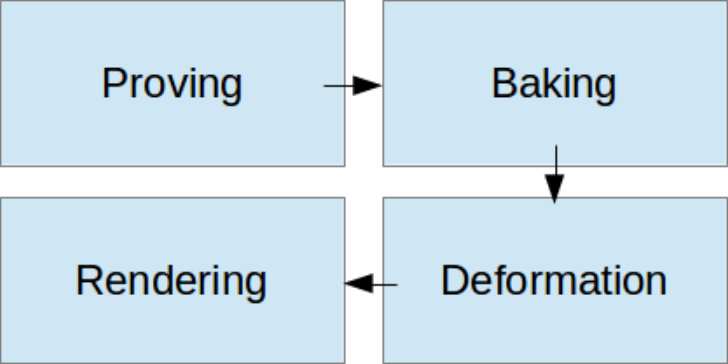
\includegraphics[scale=0.45]{pipeline.png}
\caption{Pipeline for synthetic bread making.}
\label{FigPipeline}
\end{figure}

Fig~\ref{FigPipeline} outlines our model's  pipeline. It consists of $4$ sequential stages emulating bread making. The first step introduces an algorithm for bread proving simulation. Then we apply the bread baking mathematical model \cite{Powathil2004} to slightly deform the bubbles. The third step employs Mean Value Coordinates (MVC) \cite{Floater2003} for an user defined warping of the resulting structure. Finally we apply direct volume rendering \cite{Kruger2003} getting realistic images of the process.

The proving step is defined in a $3D$ cube. We apply the baking and deformation steps to resulting $2D$ volume slices, since the baking model is cilyndrical (the properties are constant in the $Z$ coordinate).


The next subsection shows the first stage of this pipeline.

%====================================================================
\subsection{Proving simulation}
\label{breadprov}
Bubble patterns in bread result from complex processes: chemical reactions and physical deformations in bread dough. The proving step accounts for free bubble growth produced by living yeast in dough. Then, human intervention deforms dough shapes in several ways. The baking process gives the final bubbles' shape.

Phenomenological studies of bubble distribution employed X-ray tomography devices and image feature extraction \cite{Babin2006,Gonzales2008,VanDyck2014}.

To obtain structure variability, we generate bubbles distributions with a fractal-based model inspired in cheese and crater distributions \cite{Mandelbrot1982} and we validate them using the sandbox multifractal spectrum.
 We start with an sphere with initial radius of $v$ voxels and then we increment it. The number of spheres we extract from the volume in each step is proportional to the radius in the following way:

\begin{equation}
N_{spheres} = \frac{k}{r^{d}},
\end{equation}

\noindent where $k$ and $d$ are real-valued parameters, and  $r$ is the sphere radius. Fig.~\ref{FigProving} shows a $2D$ example of our model: $d$ controls the decreasing radius relationship and $k$ controls the amount of spheres we extract in each step.

Images show high resemblance in size distribution with real bread proving binarisations (see \cite{Babin2006}). We will investigate adequate parameter values to obtain fractal features similar to real bread crumbs in the validation section.


\begin{figure}
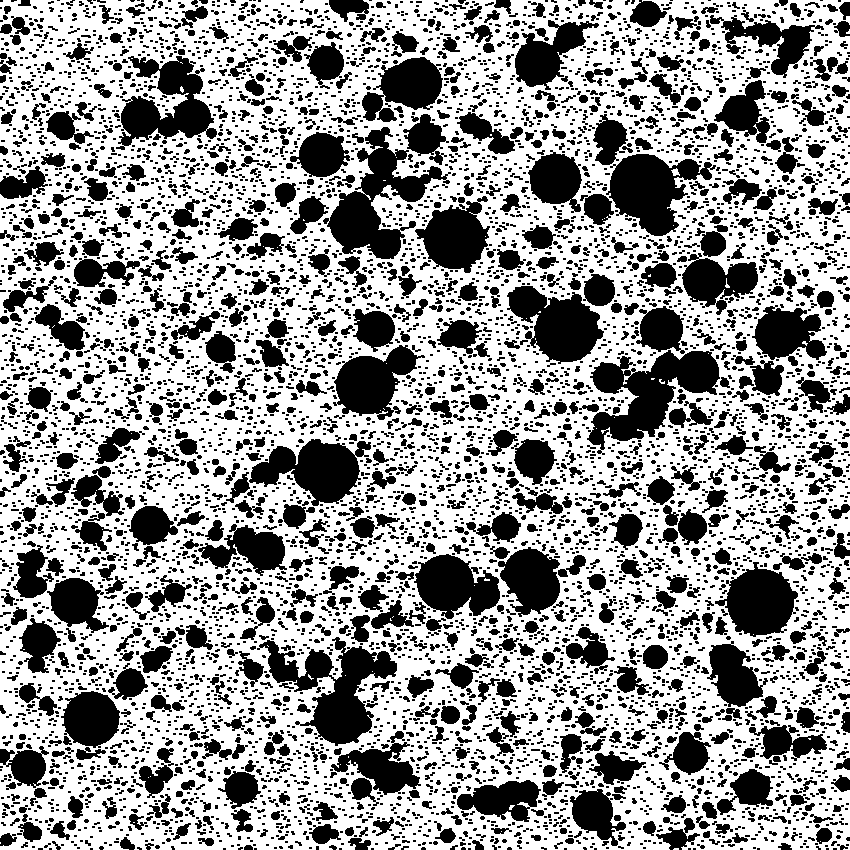
\includegraphics[scale=0.28]{bubbles.png}
\caption{Fractal bread proving simulation.}
\label{FigProving}
\end{figure}


%====================================================================
\subsection{Baking simulation}
In real bread making, baking takes place after human dough deformation. To mantain simplicity in this step, we apply it before deforming the volume: in the real case, the baking model should have arbitrary boundaries due to the external shape produced.  Our pipeline inverts baking and human deformation to mantain simplicity in the boundaries computation. The results suggest that the inversion produces low errors, obtaining adequate images for our purposes.

A simple one dimensional representation suffices \cite{Purlis2010,Powathil2004}  since the baking effect in bubbles' shape is the lowest in the bread making pipeline. 

We use the numerical implementation in \cite{Powathil2004} that is based on the finite differences scheme. The baking simulation sets an oven at $210  ^{\circ}C$ and discretises time in intervals of length $\Delta t = 0.05s$.  We obtain an array $Temp$ of $N_{grid}$ temperature values. Each value represents a dough position after $M$ baking time steps. For numerical stability, we set $N_{grid}=32$ and we interpolate the temperatures to obtain higher image resolutions ($N_{im}$).


The vector we obtained from baking has decreasing temperatures from $R = 0$ to $R = L/2$. Since the centre and the boundary of the bread has the lowest and highest temperature (heat transfer flows from the boundary to the center), $Temp[L/2]$ corresponds to $x = N_{im}/2, y=N_{im}/2$ and $Temp[0]$ corresponds to those $(x,y)$ that are away from the centre. Based on these considerations, we translate the interpolated temperatures vector $Temp_{int}$ into $2D$ coordinates using the following relationship:
\begin{align}
\displaystyle I(\frac{N_{im}}{2}-i,\frac{N_{im}}{2}-j) &= Temp_{int}[L/2-R], \\
R &= \sqrt{i^{2}+ j^{2}}, \\
i, j &\in [-\frac{N_{im}}{2},\frac{N_{im}}{2}],
\end{align}


\noindent where $R$ is the vector index, and $x$ and $y$ are $2D$ coordinates in the resulting image, {\em i.e.}, we set the image pixel $I(N_{im}/2-i,N_{im}/2-j)$ with $Temp_{int}[L/2-R]$.  The resulting image is a square of side $N_{im}$. Fig.~\ref{FigBakingVectorField} shows the result of this process.

We compute a vector field $[g_{x},g_{y}]$ from the image gradient \cite{Gonzalez2006}, and we use it to warp the volume texture in the following way:

\begin{align}
u = x+p*g_{x}[x,y],\\
v = y+p*g_{y}[x,y],
\end{align}
\noindent where $(u,v)$ are the coordinates in the warped image, ($x,y$) are the original image coordinates and $p$ is a real positive valued parameter that denotes field intensity (augmenting its value we control the baking effect on bubbles). Fig.~\ref{FigBakingVectorField} also shows the computed gradient.


\begin{figure}
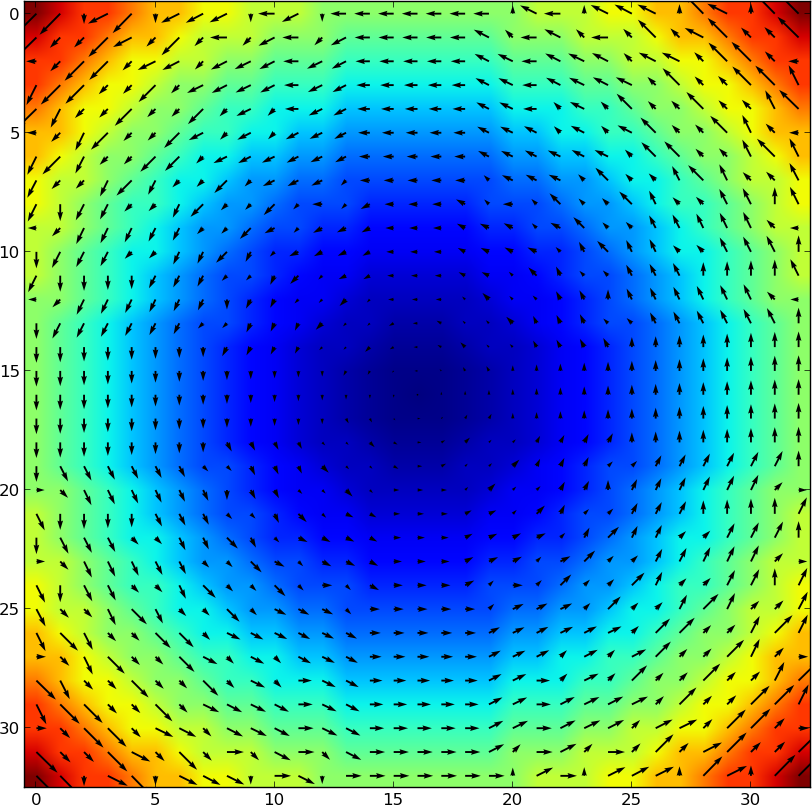
\includegraphics[scale=0.58]{vfield.png}
\caption{Temperatures from the bread baking mathematical model and superimposed gradient vector field without interpolation.}
\label{FigBakingVectorField}
\end{figure}

Arrow length indicates vector modulus. The image shows that the field's influence is higher near the crust, mostly deforming outer bubbles. This behaviour is consistent with real bread crumbs: baking influences the outer bubbles' shape, elongating them parallel to the crust \cite{Scanlon2001}, in other words, following its isotherms.

Since we defined a cilyndrical bread model, we warp each volume texture slice independently of each other, obtaining the final {\em baked} volume. Fig.~\ref{FigBaking} shows a slice result example of this process.

We should mention we tried to interpolate the resulting image instead of the original temperatures vector, but we obtained a softer vector field than expected.

\begin{figure}
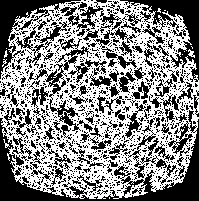
\includegraphics[scale=0.8]{baking.png}
\caption{Volume slice after baking.}
\label{FigBaking}
\end{figure}

%====================================================================
\subsection{Volume Warping}
In this stage an artist can define control points in an image, changing its external shape to produce natural bread crumb silhouettes. 


Based on our cilyndrical assumption, we apply the warp separatedly for each slice. Future work can define a $3D$ cages model for our process.


Fig.~\ref{FigMVC} shows a warping example using MVC. In that case, $11$ control points were enough to approximate the real crust shape. Fig.~\ref{FigMVCpoints} shows the control points and the deformed cage. In the example we define a higher number of control points in the region of interest (right) to produce a more controlled deformation in that region.

\begin{figure}[!ht]
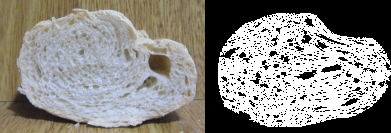
\includegraphics[scale=0.65]{warping.png}
\caption{Image warped using mean value voordinates. The image also shows a real bread image to the left. }
\label{FigMVC}
\end{figure}


\begin{figure}[!ht]
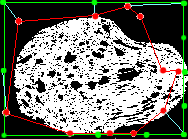
\includegraphics[scale=1.35]{warppoints.png}
\caption{Image warped, original control points (green) and moved control points (red). Other lines indicate point displacements. }
\label{FigMVCpoints}
\end{figure}


This method also warps the bubbles' shape. The deformed bubbles have a natural appearance in concordance with real bread bubbles. 


%====================================================================
%====================================================================
%====================================================================
\section{Results}
In this section we present the results of our procedural bread making pipeline and we validate the model using multifractal feature extraction.

\subsection{Rendering}
This step's purpose is the model visualization and image validation.

Direct volume rendering (DVR) \cite{Kruger2003,Levoy1988, Max1995} approximates the light transport equation by throwing rays into a volume from a virtual camera, accumulating density information. The process forms an image from a camera positioned in space.

We prefer DVR over other state-of-the-art methods such as Ray Tracing \cite{Whitted1980,Singh2010}, Path Tracing \cite{Lafortune1993} and Photon Mapping \cite{Jensen1996}, since they are computationally expensive and they require a detailed object mesh.

Fig.~\ref{FigRenders} shows DVR-rendered images  of $3D$ volumes we obtained in this work. Images show a realistic bread crumb appearance, suitable for photo-realistic rendering and serious games \cite{Susi2007}. Fig.~\ref{FigRenders2} shows breads with crust. We artificially added the crust to the borders of the bread.

\begin{figure}[!ht]
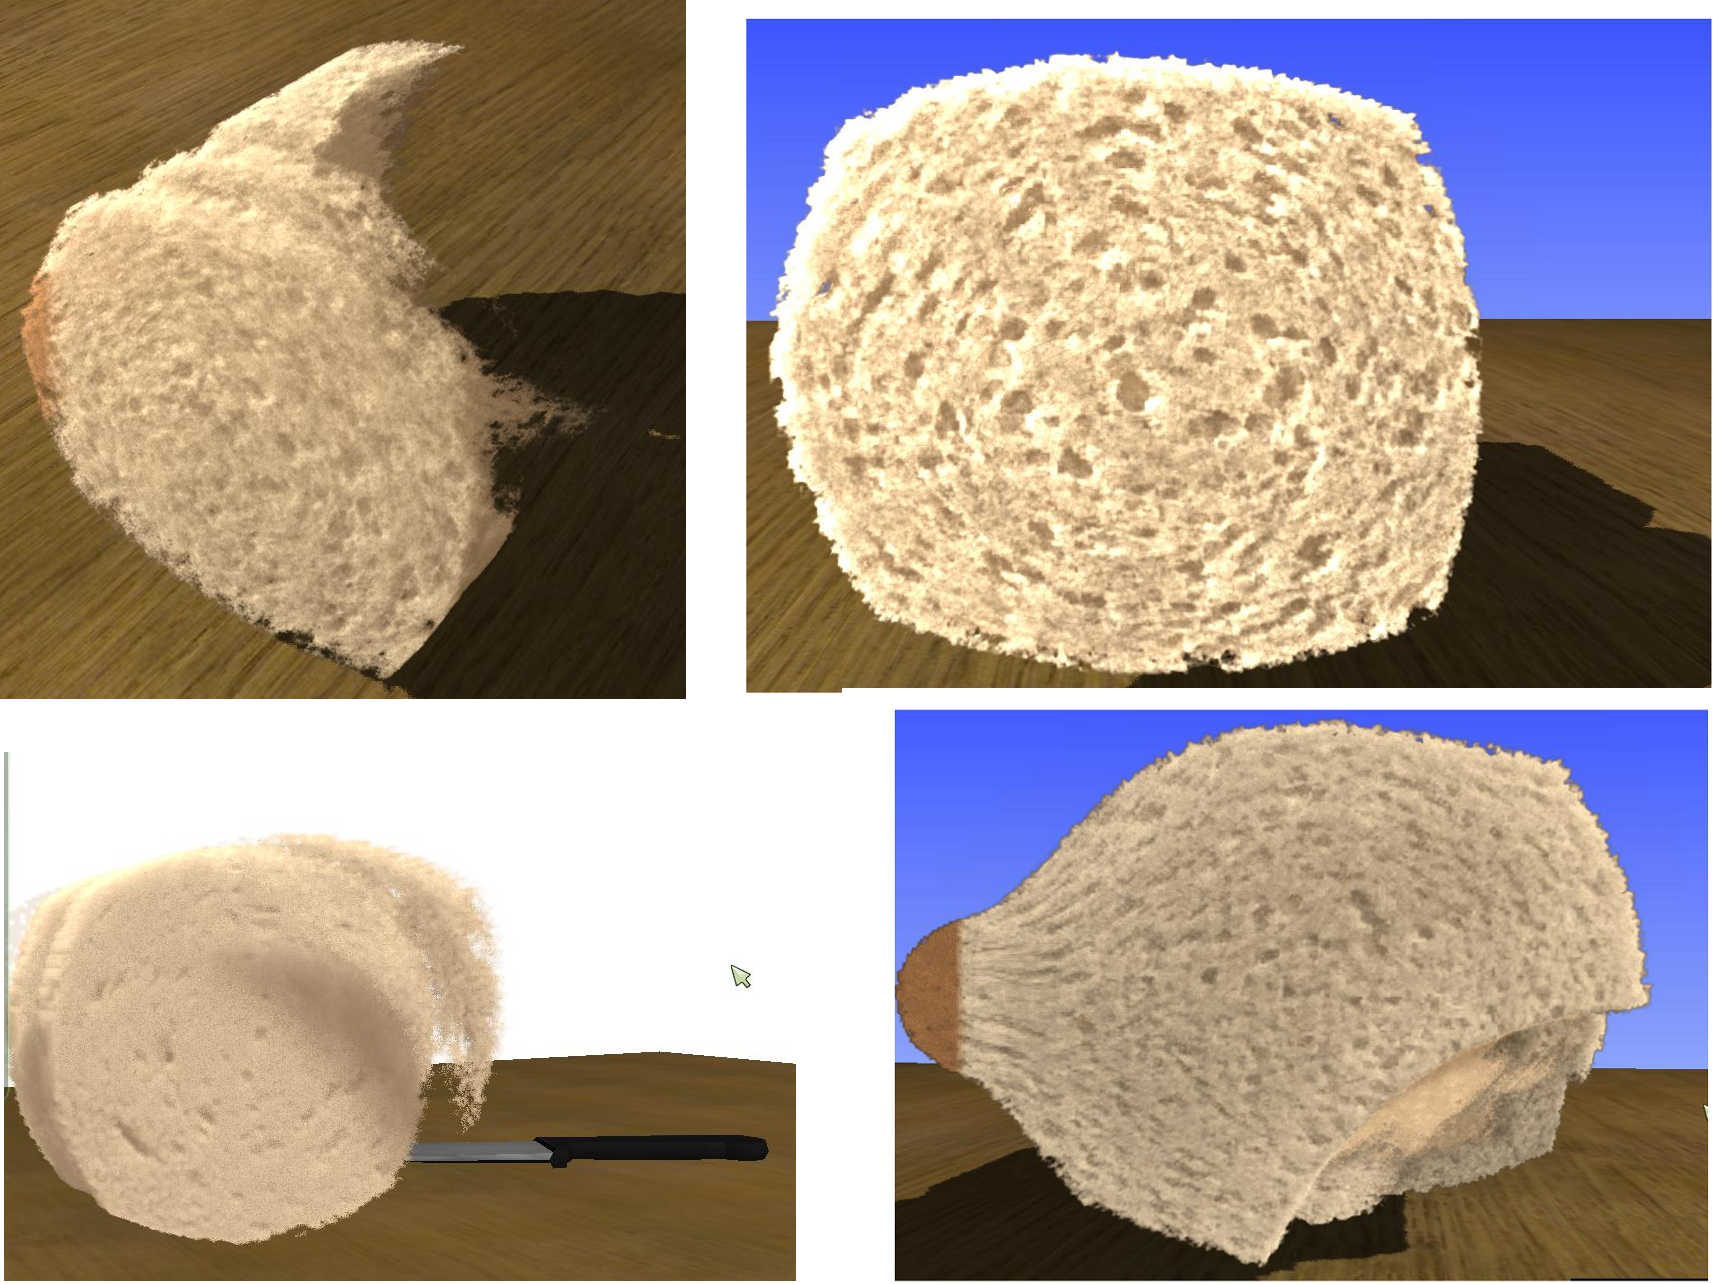
\includegraphics[scale=0.15]{render2.png}
\caption{DVR synthetic bread crumb renders}
\label{FigRenders}
\end{figure}

\begin{figure}[!ht]
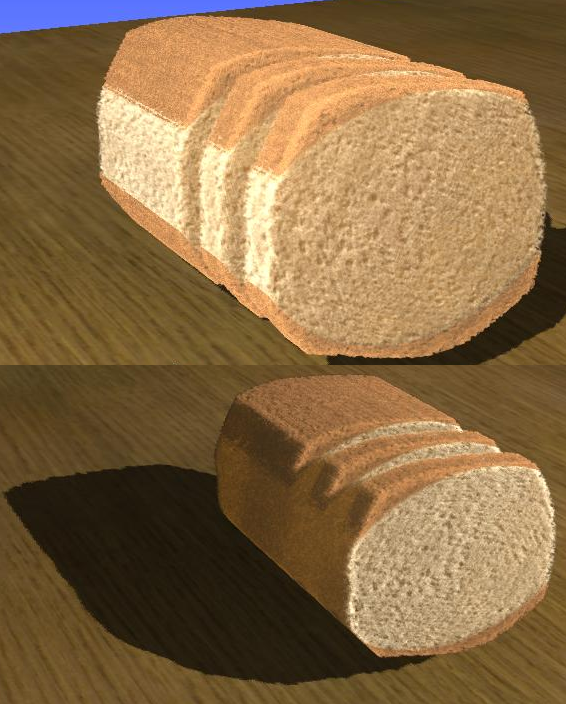
\includegraphics[scale=0.35]{crusts.png}
\caption{DVR synthetic bread crumb renders with crust}
\label{FigRenders2}
\end{figure}

The authors have used physically correct mathematical models constructing a multi-step pipeline in synthetic bread crumb modelling and visualization. 

Next section validates this model using fractal methods.

%====================================================================
\subsection{Model Validation}

We apply the sandbox multifractal method to study the geometry we obtained after the deformation step. This method is best suited for geometrical characterisation than other multifractal approaches.

We apply the sandbox method to $10$ binarised real bread crumb images that we captured with a digital camera and $10$ syhthetic images produced using our pipeline, after the deformation step, obtaining $20$ feature vectors. Then we separate each class and we compute boxplots for the two classes. We manually segmented real bread crumbs to prevent automatic segmentation errors as in \cite{Bosch2011}. The model has $5$ parameters:


\begin{align}
N_{spheres} &= \frac{k}{r^{d}},\\ r &= v_{min}+step*j, j \in [0,\frac{v_{max}}{step}]
\end{align}
$k,d,v_{min},v_{max}$ and $step$ that controls bubble's generation in the proving stage. We implemented an automated search in parameter space and we found that the following parameters produce the lowest error:

\begin{align*}
k &= 0.07 \frac{N_{x}\times N_{y}\times N_{z}}{20} ,\\
d &=2.78,\\
v_{min} &=2,\\
v_{max} &=20.\\
step &=1,
\end{align*}
\noindent where $N_{x}$, $N_{y}$ and $N_{z}$ are the proving volume dimensions in each spatial coordinate. The accumulated error in medians is $\sim 0.21$ meaning a mean error of $0.21/21 \sim 0.01$  in each dimension. We compute this error as:

\begin{equation}
Error = \displaystyle \sum abs(means_{real}-means_{synthetic}).
\end{equation}
Fig.~\ref{bestboxplot} shows boxplots of real and synthetic breads with the medians for each dimension joined by dashed lines. When $q < 0$ dimensions have a higher dispersion, since the method approximates these dimensions less accurately. The figure shows almost identical spectra for real and synthetic breads.  Fig.~\ref{realbin} and  Fig.~\ref{bestwarp} show an example of real and synthetic binarisations for these parameters.

\begin{figure}[!ht]
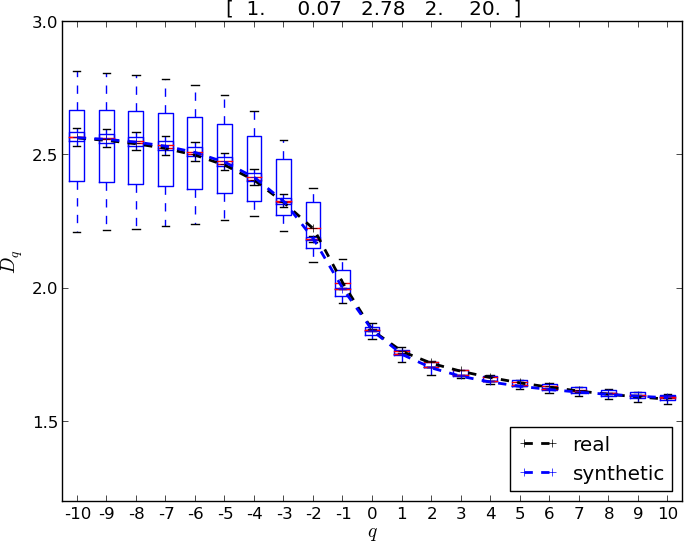
\includegraphics[scale=0.5]{bestboxplot.png}
\caption{Best fitting parameters. The total error in medians is $\sim 0.21$.}
\label{bestboxplot}
\end{figure}

\begin{figure}[!ht]
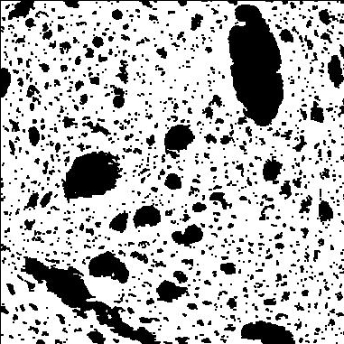
\includegraphics[scale=0.2]{realbin.png}
\caption{ Real bread and binarisation example.}
\label{realbin}
\end{figure}

\begin{figure}[!ht]
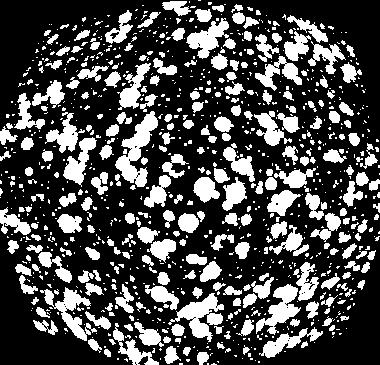
\includegraphics[scale=0.2]{bestwarp.png}
\caption{Model distribution example showing similar multifractal features to real breads.}
\label{bestwarp}
\end{figure}


Automated searchs in parameter space may be useful to automatically match other bread types and materials.

%To test the rendering algorithm, we employ the Multifractal Spectrum (MFS) \cite{Xu2009}. This method can distinguish bread crumb from non-bread crumb images with high accuracy  \cite{Baravalle2012}.

%SOM maps \cite{Kohonen2001} reduces the N-dimensional feature space into a two dimensional representation while mantaining neighborhood information. These maps allow to see feature vectors distributions in space in a human-useful representation.

%Fig.~\ref{FigSOM} shows the SOM map for the MFS image representation. We compute the MFS in the $80$ images obtaining a feature vector for each of them. We use these vectors to populate the map. The map we obtained presents evidence for bread and non-bread separability since each class' vectors is separable.

%\begin{figure}[h!]
%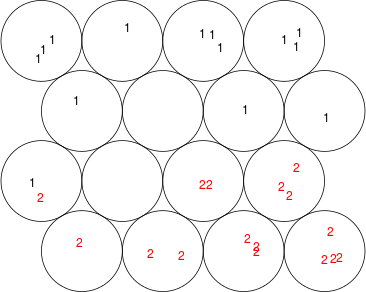
\includegraphics[scale=0.65]{som.png}
%\caption{Self Organising Maps showing bread and non-bread separability. 1: Bread, 2: Non-bread }
%\label{FigSOM}
%\end{figure}

%The test is as follows: $20$ real bread crumb images captured with a digital camera and $20$ non-bread images from a public dataset \cite{FeiFei2004} train a Random Forests (RF) \cite{Breiman2001} and Support Vector Machines (SVM) \cite{Vapnik1995} defining $2$ balanced classes. Twenty synthetic images obtained using our method and $20$ non-bread images from the same public dataset defines the test set.


%Table~\ref{Table1} shows the classifiers' performance (the percentage of correct classifications in the test set). Table~\ref{Table2} shows the SVM classifier confusion matrix: each row represents the correct class, and each column the classifier result; a diagonal matrix means the classifier performed optimally.

%\begin{table}[htb]
%\centering
%\begin{tabular}{c|c}
%\hline
 %Method & Accuracy  \\
%\hline
% RF & 77.5 \% \\
%SVM  & 87.5 \% \\
%\hline
%\end{tabular}
%\caption{Classification performance }
%\label{Table1}
%\end{table}

%\begin{table}[htb]
%\centering
%\begin{tabular}{c|c|c}
%\hline
% Class & bread & non-bread  \\
% \hline
%bread & 18 & 2  \\
% non-bread & 3 & 17  \\
 %\hline
%\end{tabular}
%\caption{Confusion matrix for the SVM classifier}
%\label{Table2}
%\end{table}

%\begin{table}[htb]
%\centering
%\begin{tabular}{c|c|c}
%\hline
% Class & bread & non-bread  \\
 %\hline
%bread & 13 & 7  \\
% non-bread & 2 & 18  \\
 %\hline
%\end{tabular}
%\caption{Confusion matrix for the random forests classifier}
%\label{Table3}
%\end{table}

%An automatic robust classifiers classify most synthetic bread images as real bread images (the classifiers detected $2$ and $7$ as synthetic).

Based on this test, we strongly believe that our procedure adequately models bread crumbs structures. The sandbox multifractal method %and the MFS
detects compatible fractal patterns in our synthetic images and in real bread crumbs, suggesting the correctness of the bubble size distributions' model.


%====================================================================
%====================================================================
%====================================================================
\section{Discussion}
We introduced a pipeline to model realistic bread crumb geometry based on a fractal generation procedure. The $4$ different stages flexibilised the model, allowing to tune and test each of them separatedly.

We designed the proving step inspirated in the visual similarities we found with Mandelbrot's model for moon's craters and cheeses air bubbles. These patterns can be used in several other materials involving bubbles such as foams and sponges. The main visual difference with real bread crumbs were the self-avoiding bubbles in bread. An algorithm with this enhancement will have higher modeling and computing costs. We defined different parameters related to the bubble radius, amount and its relationship.

The original baking model is $1D$. We used the temperatures information  and we translated them to $2D$ coordinates using euclidean distance to the $2D$ coordinates origin. We defined a cilyndrical $3D$ model setting constant properties for the $Z$ coordinate. 

The baking-deformation inversion we introduced eliminates the necessity of $3D$ baking models, reducing the model complexity and the computing resources consumed. The $2D$ simplification of the kneading step agreed with our cilyndrical model and presented acceptable results in bubble global and local deformations. This  deformation limitation can be extended to $3D$ in a future work. The MVC method performed the deformations intuitively.

We performed a test to validate the model after deformation. The test used the Sanbox method, best suited for geometrical multifractals, and obtained synthetic spectra with low error rates when compared to real spectra.  These results indicates that the bubble's proving model and the baking and deformation stages generate bubble distributions that concordates with real bread crumbs bubbles distribution (amounts and sizes of bubbles). 
We found higher dispersion in the negative dimensions ($q \ge 0$), since the method better approximates the positive generalised multifractal dimensions. 

%The second test employed the MFS to validate the suitability of the pipeline in a typical rendering system. We also obtained low error rates in classification performance using two different classifiers. The SOM maps of the feature space shows the separability of bread and nonbread images. This indicates our rendering system is producing synthetic images with multifractal features similar to real bread crumbs. We only found a high error rate for synthetic breads (they were classified as synthetic) using the RF classifier ($7$ out of $20$), but this limitation might be a consequence of a particular incapacity of the RF classifier in the synthetic samples, since the SVM classifier  (and the SOM maps) performed better. The rendering algorithm should be refined and more tests are needed to obtain lower error rates for this classifier.

A more detailed link between bread crumb physical features (coarseness, porosity) and multifractal features is needed for better understanding of the spectrum's dimensions. It will also be useful for procedural model generation \cite{Baravalle2012}. Further analysis might be useful for richer characterisations

The use of a DVR engine produces realistic images and allowed to test the suitability of our model. Other photo-realistic algorithms can be used to test the capabilities of our method.


%====================================================================
%====================================================================
%====================================================================
\section{Conclusions and future work}


To the best of the authors' knowledge, this is the first attempt in computer graphics to model the bread crumb geometry using a mathematical model of bread baking and other bread making steps. The problem's complexity, which in certain cases has exceeded available computing capabilities, produced that few work appeared in the literature. With the advenement of GPGPU, more realistic models appeared for other materials. We thought our model may be the first one in a future line of research in bread modeling in computer graphics. 

We proposed and validated a flexible and powerful pipeline to procedurally model bread crumbs. This is a contribution to the state of the art since typical approaches for modeling the geometry of bread crumbs involve advanced tomography equipment \cite{VanDyck2014} or artistical considerations \cite{Cho2007}. The images we obtained and the tests we performed  suggests the correctness of the model, suitable for application in $3D$ engines, serious games and photo-realistic rendering.

Artists can model the bread crumb global shape using control points in a plane. Bubbles naturally follow this shape, accurately emulating bread crumb bubbles.

We employed fractal and machine learning methods to model and validate our procedure. The low error rates we obtained make us beleive that the bubbles' size distribution is accurate in a (multi) fractal sense: the number, sizes and shape of the bubbles concordate with real bread crumbs. Also, since we mathematically emulated key steps in bread making, we obtained natural shapes for bubbles that adapt to the bread exterior silhouette, producing mathematically correct patterns.

As possible continuations, we will define interfaces for visual interaction with the control points, and a complete $3D$ model for deformation. We may extend the proving method introducing spheres that self avoids. We plan to perform further tests on our classification procedure to gain insight in multi-fractal bread features.


%% The Appendices part is started with the command \appendix;
%% appendix sections are then done as normal sections
%% \appendix

%% \section{}
%% \label{}

%% References
%%
%% Following citation commands can be used in the body text:
%% Usage of \cite is as follows:
%%   \cite{key}          ==>>  [#]
%%   \cite[chap. 2]{key} ==>>  [#, chap. 2]
%%   \citet{key}         ==>>  Author [#]

%====================================================================
%====================================================================
%====================================================================
%% References with bibTeX database:
\bibliographystyle{model3-num-names}
\bibliography{bib}

%% Authors are advised to submit their bibtex database files. They are
%% requested to list a bibtex style file in the manuscript if they do
%% not want to use model3-num-names.bst.

%% References without bibTeX database:

% \begin{thebibliography}{00}

%% \bibitem must have the following form:
%%   \bibitem{key}...
%%

% \bibitem{}

% \end{thebibliography}


\end{document}

%%
%% End of file `elsarticle-template-3-num.tex'.